\chapter{The results, and how to read each figure}\label{ch:results}

The numbers are in \file{RESULTS.md}; this chapter teaches you to \emph{read} the figures, which is what a committee will test.

\section{H1: repliers downvote the comment they answer}
\begin{figure}[h]
\centering
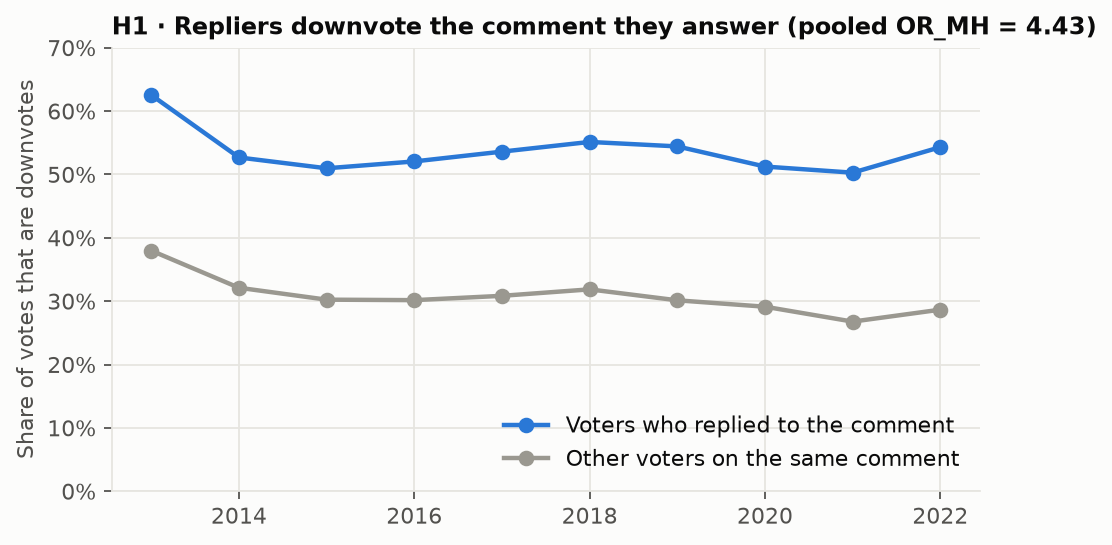
\includegraphics[width=0.85\textwidth]{04_h1_by_year.png}
\caption{H1 by year. Blue: share of downvotes among repliers' votes. Grey: among other voters on the same comments.}\label{fig:h1}
\end{figure}
\begin{readbox}
Each point is a year. The vertical gap between blue and grey is the effect in percentage points, about 20--25 points. Both lines move together (a downward step after 2013 and a slight rise afterwards), which means the \emph{overall mood} changes by year but the gap is stable. The shares are pooled shares; the title's 4.43 is the comment-stratified odds ratio, a different summary of the same pattern.\end{readbox}

\section{H2: the dyad analysis}
\begin{figure}[h]
\centering
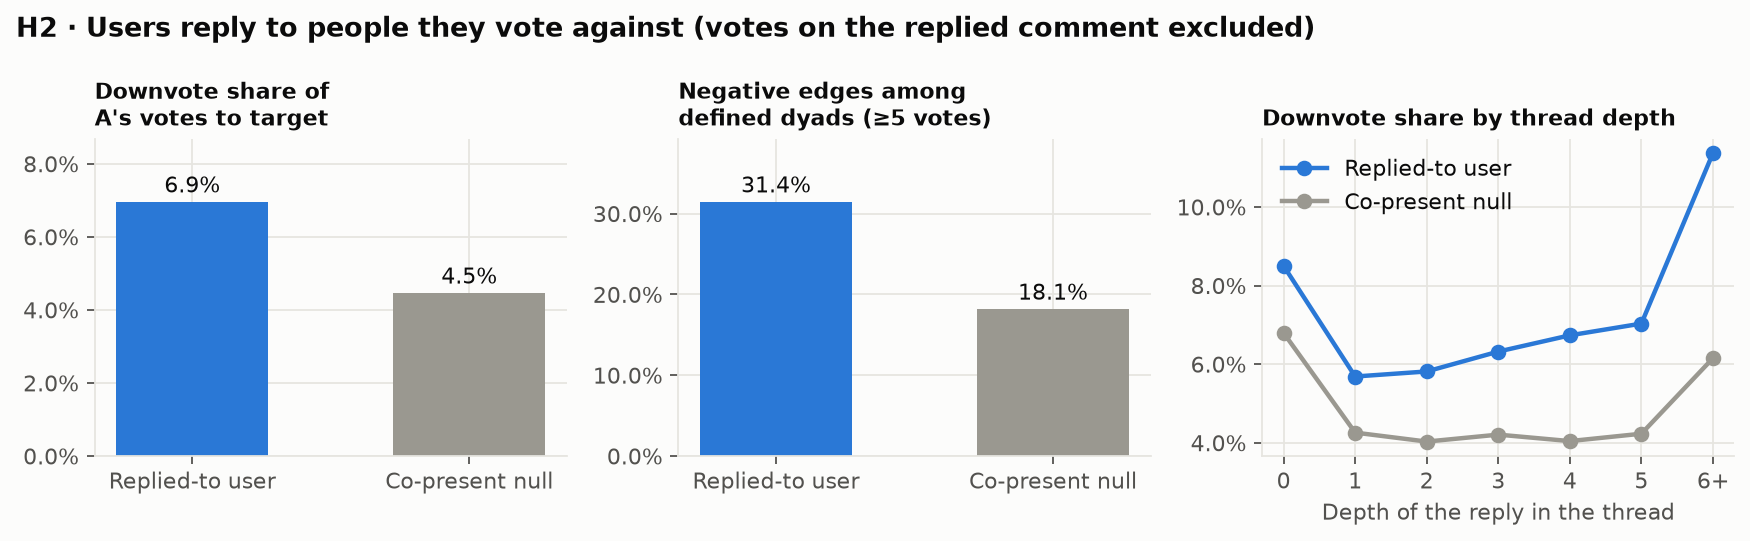
\includegraphics[width=\textwidth]{05_h2_dyad.png}
\caption{H2 with votes on the replied comment excluded. Left: $A$'s downvote share toward the target. Middle: share of negative edges among defined pairs. Right: downvote share by thread depth.}\label{fig:h2}
\end{figure}
\begin{readbox}
\textbf{Left:} 6.9\% against 4.5\% of $A$'s votes to the target are downvotes: low in absolute terms because most votes everywhere are upvotes, but 50\% higher in relative terms. \textbf{Middle:} the share of \emph{pairs} classified as negative: 31.4\% against 18.1\%. Remember that this panel uses only pairs with $\ge5$ votes (Section~\ref{sec:h2}). \textbf{Right:} the gap exists at every depth, and both lines rise for deeper replies (deeper conversations are more combative); the last point (6+) is pooled and based on fewer replies.
\end{readbox}

\section{Lifetime: CCDF and Kaplan--Meier}
\begin{figure}[h]
\centering
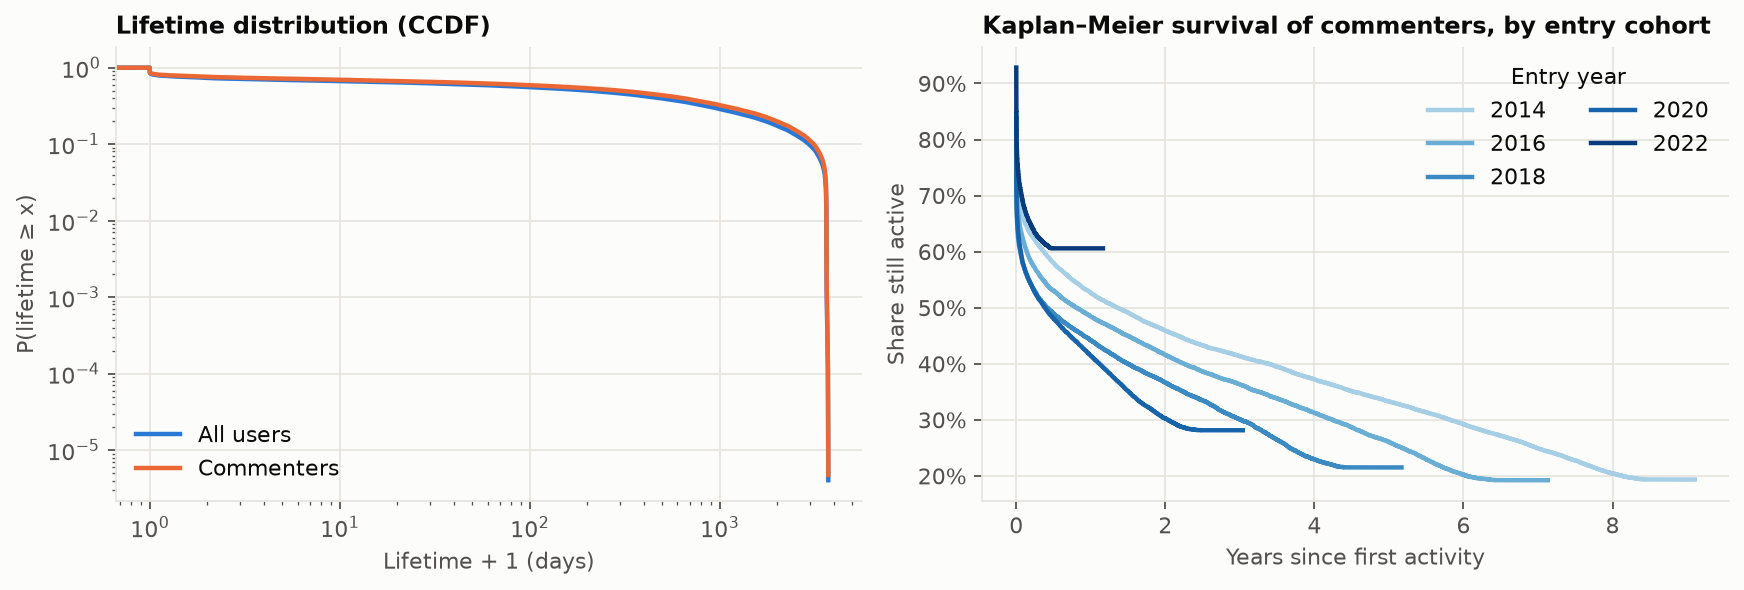
\includegraphics[width=\textwidth]{06_lifetime_ccdf_km.png}
\caption{Left: complementary cumulative distribution of lifetimes (log--log). Right: Kaplan--Meier survival by entry cohort.}\label{fig:km}
\end{figure}
\begin{readbox}
\textbf{Left:} a CCDF gives, for each $x$, the share of users with lifetime at least $x$; on log--log axes a straight line would mean a power law. Here the curve drops at 1 day (the 26.7\% one-day users), is nearly flat for a long time and falls sharply at about ten years, where the window ends. That final cliff is the window, not a behaviour. \textbf{Right:} each curve starts at 100\% and steps down when users leave. Steep initial drops are first-weeks churn. Curves end where the cohort's observation ends, and they \emph{flatten at the end} because the remaining users are censored and no longer counted as at risk. Later cohorts are lower: users who joined in 2018 or 2020 leave faster than those who joined in 2014. The 2022 cohort is short and mainly shows early churn.
\end{readbox}

\section{H4: the Cox model}
\begin{figure}[h]
\centering
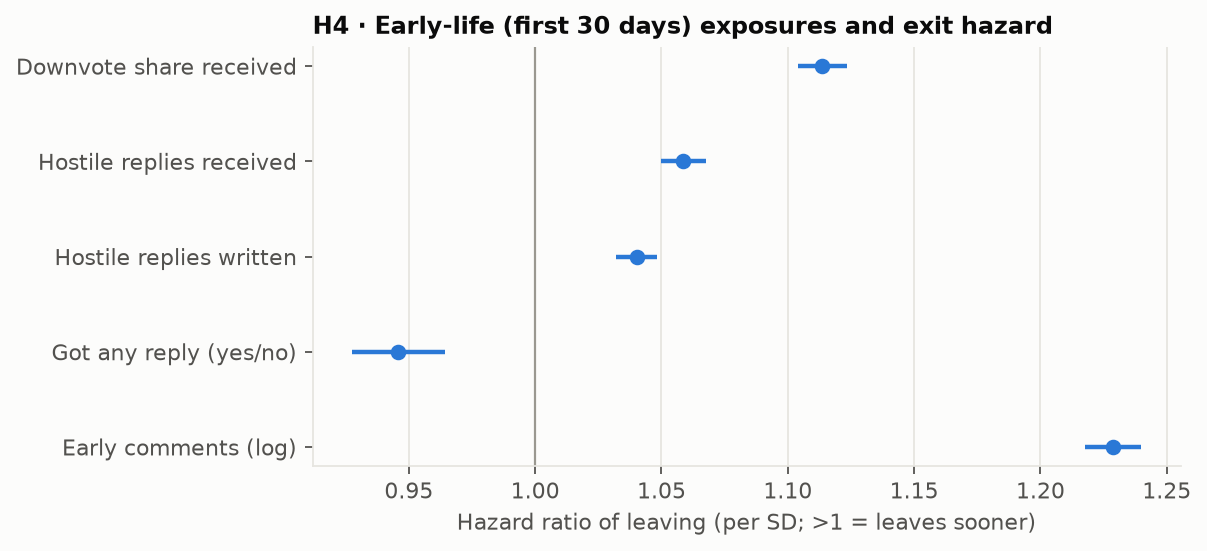
\includegraphics[width=0.9\textwidth]{06_h4_cox.png}
\caption{Hazard ratios of leaving per standard deviation of each early exposure; bars are 95\% intervals.}\label{fig:cox}
\end{figure}
\begin{readbox}
The vertical grey line is a ratio of 1 (no association). To the right of it, a higher value of the covariate goes with leaving sooner; to the left, later. Downvote share received (1.11) and hostile replies received (1.06) go with leaving sooner; getting any reply (0.95) with staying longer. The largest ratio is for the number of early comments (1.23), which is mostly an intensity signal. Intervals are narrow because of 98,670 users; their width does not tell you about bias.
\end{readbox}

\section{Multiverse}
\begin{figure}[h]
\centering
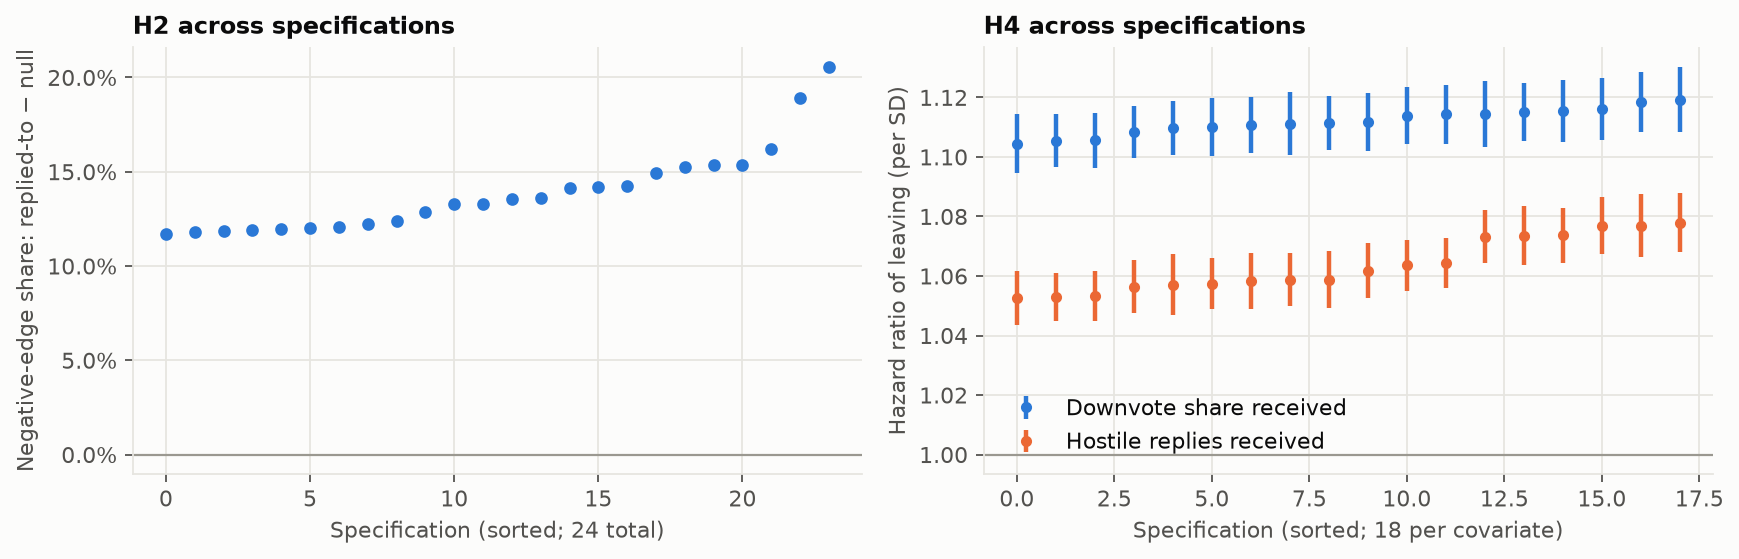
\includegraphics[width=\textwidth]{07_multiverse.png}
\caption{Left: H2 difference real $-$ null across 24 specifications, sorted. Right: H4 hazard ratios across 18 specifications.}\label{fig:multiverse}
\end{figure}
\begin{readbox}
Each dot is one analysis with a different combination of arbitrary choices. Dots are \emph{sorted by size}, so the x axis is an index, not a variable. What matters is whether any dot crosses zero (H2) or 1 (H4): none does. The spread of H2, 11.7 to 20.6 points, is an honest statement of how much the headline depends on the choices. The H4 ratios are tight because the specifications differ only in early window, churn buffer and shrinkage.
\end{readbox}

\section{Positive votes}
\begin{figure}[h]
\centering
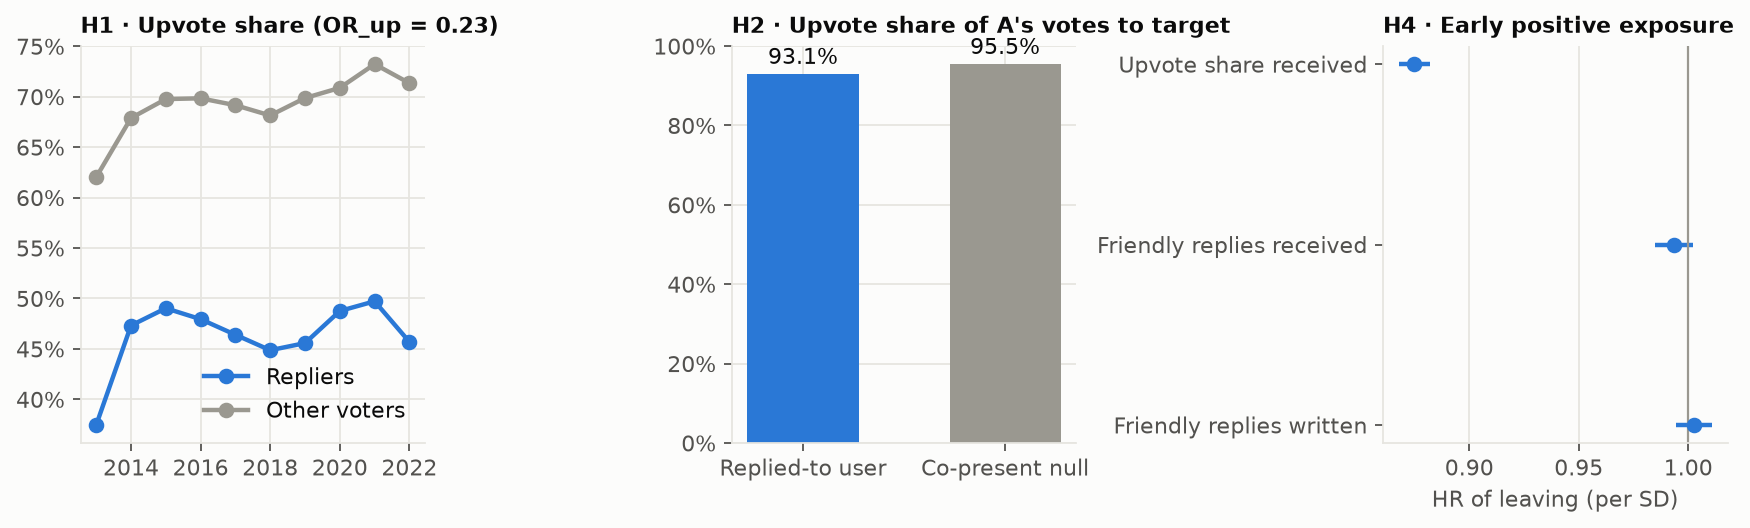
\includegraphics[width=\textwidth]{08_positive_votes.png}
\caption{Mirror of H1, H2 and H4 for positive votes.}\label{fig:pos}
\end{figure}
\begin{readbox}
Left: the mirror image of Figure~\ref{fig:h1} (repliers upvote less). The two figures contain the same information; do not count them as two findings. Middle: near ceilings (93\% against 95.5\%), so the same relative difference looks small. Right: only the upvote share received has a clear association with leaving (HR 0.87: more upvotes, later exit). Friendly replies are at 1.
\end{readbox}

\section{Long-lived users}
\begin{figure}[h]
\centering
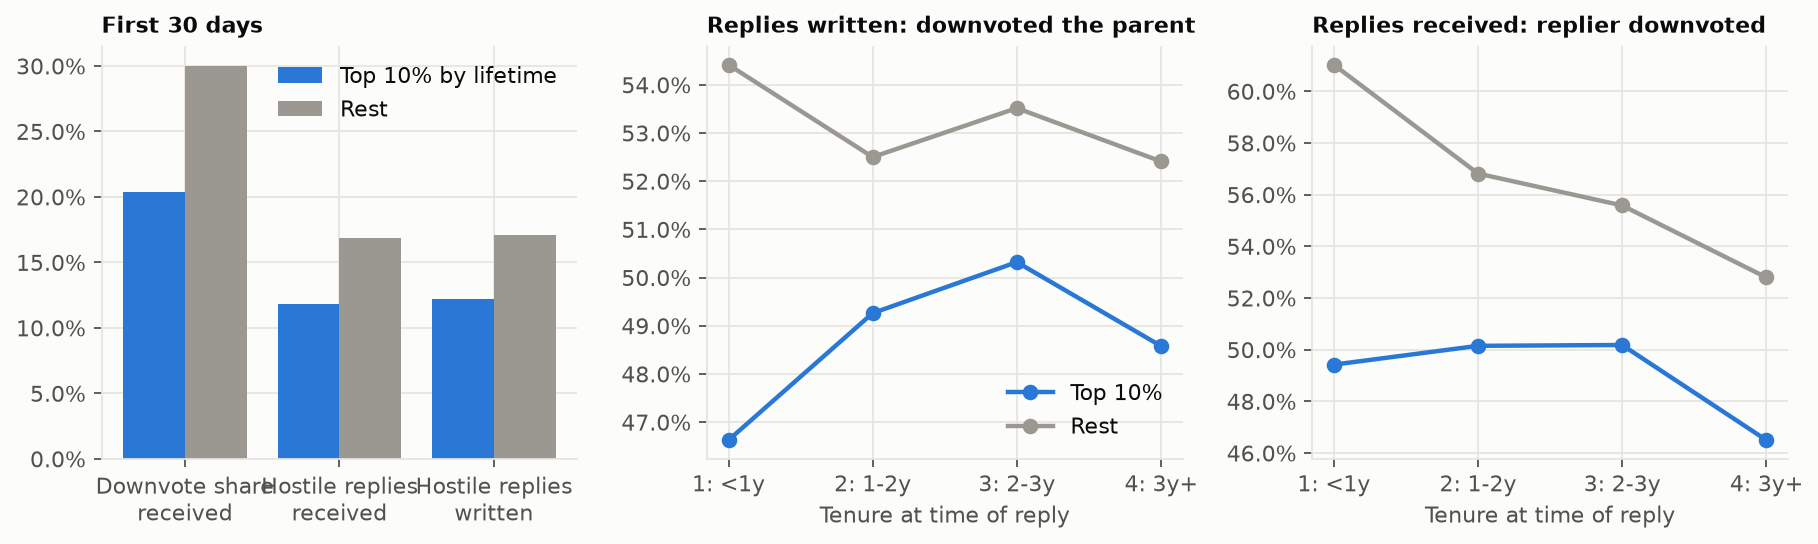
\includegraphics[width=\textwidth]{09_top_decile.png}
\caption{Top 10\% by lifetime within cohort versus the rest.}\label{fig:top}
\end{figure}
\begin{readbox}
Left: in the first 30 days the long-lived group receives fewer downvotes and fewer hostile replies, and writes fewer. Middle and right: by tenure at the time of the reply, the long-lived group less often downvotes the parent it answers (about 47--50\% against 52--54\% for the rest), and the replies it receives less often come from downvoters (46--50\% against 53--61\%). The curves of the rest fall with tenure on the right panel, the long-lived group's is flat. Read with Section~\ref{sec:longlived}: the group is mostly censored survivors.
\end{readbox}

\section{Which sentences the results do and do not allow}
\begin{tabularx}{\textwidth}{@{}Y Y@{}}
\toprule
Allowed & Not allowed \\
\midrule
``Users who reply to a comment downvote it more than other voters on that comment.'' & ``Replying is an act of opposition'' (no text; different voters) \\
``Real reply pairs are more often negative than co-present random pairs.'' & ``Users seek out opponents'' (article-level null is easy to beat) \\
``Early downvote exposure is associated with leaving sooner.'' & ``Downvotes cause users to leave'' (observational, untimed votes) \\
``The direction is stable across 24 and 18 specifications.'' & ``The effect is jointly significant across specifications'' (not tested) \\
``The long-lived group's first month looked less hostile.'' & ``Calm newcomers become long-lived'' (selected group) \\
\bottomrule
\end{tabularx}
